
\section{Dataset}
To build our predictive models, we use a dataset collected by urologists at UCLA, which has previously been used in publication\cite{gore}.  This data follows a cohort of roughly 1000 patients who received one of 3 possible treatments - prostatectomy, radiation therapy, or brachytherapy for a period of 5 years.  Surveys were sent at various time points after treatment that asked patients to assign a functional score in each of several categories: sexual, bowel, and urinary function, as well as general physical and mental well being.  These scores are between 0 and 100.  Several patient attributes such as age, race, comorbidity count, and PSA level were also recorded for every patient.  Figure 1 shows an example of the average sexual function scores in the entire dataset after each of 3 treatments.

\section{General Shape of Function Curves}
The very first thing we did was to see on average what the function curves looked like for different patients, and whether they differed by treatment.  Below, for each of the 3 side effects, we plot the aggregate function time series for patients opting for each treatment.  

\begin{figure}
\centering
\begin{subfigure}[bowel function]{
  \includegraphics[width=.3\linewidth,height=0.3\textheight]{/Users/glareprotector/prostate_git/glare/tex_files/sections/explore/avg_time_series_by_treatment/bowel_func.png}}
\end{subfigure}
\begin{subfigure}[sexual function]{
  \includegraphics[width=.3\linewidth,height=0.3\textheight]{/Users/glareprotector/prostate_git/glare/tex_files/sections/explore/avg_time_series_by_treatment/sexual_func.png}}
\end{subfigure}
\begin{subfigure}[urinary function]{
  \includegraphics[width=.3\linewidth,height=0.3\textheight]{/Users/glareprotector/prostate_git/glare/tex_files/sections/explore/avg_time_series_by_treatment/urin_func.png}}
\end{subfigure}
\caption{Average patient time series for the 3 side effects, stratified by treatment}
\end{figure}

All of the aggregate curves seem to have a similar shape: an initial instantaneous drop off in function level, followed by a rise to some steady state function level.  This hints that we should model the curves parametrically, parameterizing the key attributes of it - the initial drop, the long-term drop, and the rate of function recovery.  Secondly, the treatment chosen does seem to affect the level of initial function drop and long term function level.

\section{Dependence of Function Curves on Patient Attributes}

The second thing we wanted to look at was for a given side effect and treatment, whether the function curves vary depending on the available attributes.  Below, for each of the 3 side effects, for each of the 6 attributes we have for patients, divide the dataset into 2 halves, based on the given attribute.  We plot the average function time series for each half of the dataset, to see if there is a difference.

\begin{figure}
\begin{subfigure}[bowel function]{
  \includegraphics[width=.3\linewidth,height=0.3\textheight]{/Users/glareprotector/prostate_git/glare/tex_files/sections/explore/avg_time_series_strat_by_attribute/bowel_func.png}}
\end{subfigure}
\begin{subfigure}[sexual function]{
  \includegraphics[width=.3\linewidth,height=0.3\textheight]{/Users/glareprotector/prostate_git/glare/tex_files/sections/explore/avg_time_series_strat_by_attribute/sexual_func.png}}
\end{subfigure}
\begin{subfigure}[urinary function]{
  \includegraphics[width=.3\linewidth,height=0.3\textheight]{/Users/glareprotector/prostate_git/glare/tex_files/sections/explore/avg_time_series_strat_by_attribute/urin_func.png}}
\end{subfigure}
\caption{Average patient time series for the 3 side effects, stratified by each of 6 patient attributes}
\end{figure}

It seems like there is a difference in the curves, depending on various attributes.  However, the attributes seem to be strongly correlated with the pre-treatment function level.  It seems logical that the pre-treatment state would be highly correlated with the post-treatment function level.  To verify this, we make the same plots as before, except this time, we stratify the patients by their pre-treatment function level.  Indeed, pre and post-treatment function levels are highly correlated.


\begin{figure}
\begin{subfigure}[bowel function]{
  \includegraphics[width=.3\linewidth,height=0.2\textheight]{/Users/glareprotector/prostate_git/glare/tex_files/sections/explore/avg_time_series_strat_by_pre_state/bowel_func.png}}
\end{subfigure}
\begin{subfigure}[sexual function]{
  \includegraphics[width=.3\linewidth,height=0.2\textheight]{/Users/glareprotector/prostate_git/glare/tex_files/sections/explore/avg_time_series_strat_by_pre_state/sexual_func.png}}
\end{subfigure}
\begin{subfigure}[urinary function]{
  \includegraphics[width=.3\linewidth,height=0.2\textheight]{/Users/glareprotector/prostate_git/glare/tex_files/sections/explore/avg_time_series_strat_by_pre_state/urin_func.png}}
\end{subfigure}
\caption{Average patient time series for the 3 side effects, stratified by each of 6 patient attributes}
\end{figure}


We wonder whether after controlling for the pre-treatment state, a patient's attributes still impact their curves.  Thus, for each side effect, treatment combination, for each of the 6 attributes, we made a scatter plot of the attribute vs the change in side effect function level before treatment and right after treatment (at the 1 month survey time).  There are too many side effect/treatment combinations to display scatter plots for, but below, we choose 3 such combinations and show their associated scatter plots.

\begin{figure}
\begin{subfigure}[bowel function/brachytherapy]{
  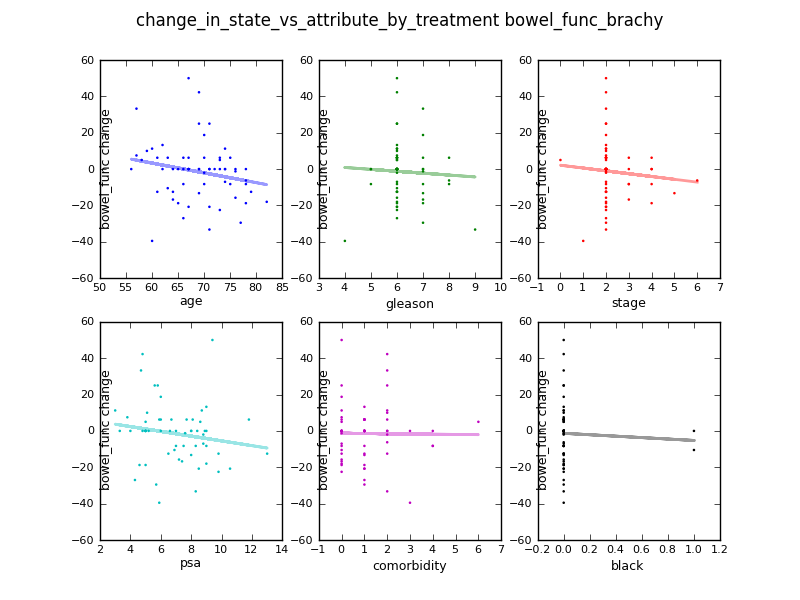
\includegraphics[width=.3\linewidth,height=0.2\textheight]{/Users/glareprotector/prostate_git/glare/tex_files/sections/explore/change_in_state_vs_attribute_by_treatment/bowel_func_brachy.png}}
\end{subfigure}
\begin{subfigure}[sexual function/surgery]{
  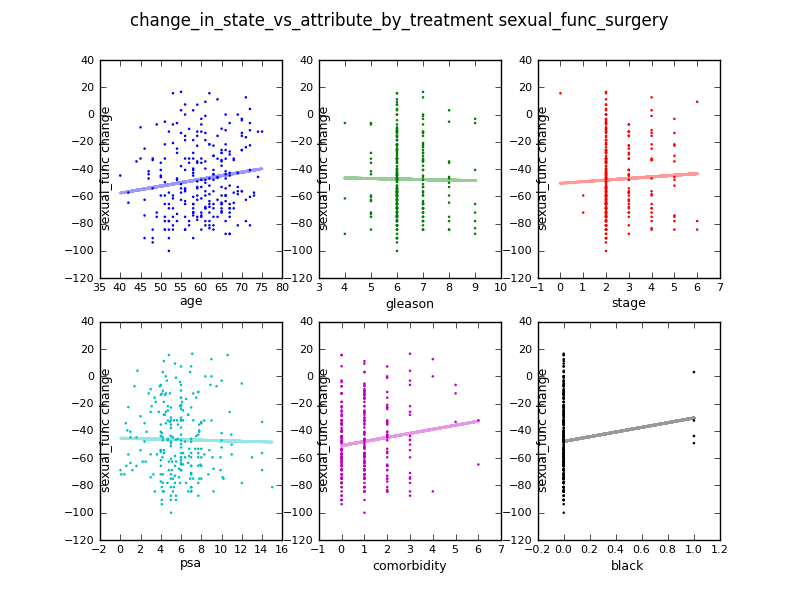
\includegraphics[width=.3\linewidth,height=0.2\textheight]{/Users/glareprotector/prostate_git/glare/tex_files/sections/explore/change_in_state_vs_attribute_by_treatment/sexual_func_surgery.png}}
\end{subfigure}
\begin{subfigure}[urinary function/radiation]{
  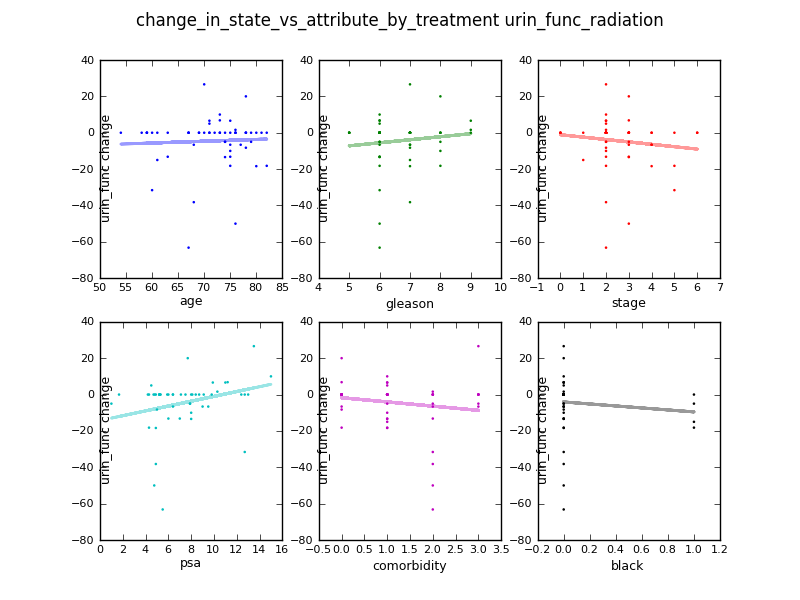
\includegraphics[width=.3\linewidth,height=0.2\textheight]{/Users/glareprotector/prostate_git/glare/tex_files/sections/explore/change_in_state_vs_attribute_by_treatment/urin_func_radiation.png}}
\end{subfigure}
\caption{Initial drop in function level vs attribute, for 3 side effect/treatment combinations}
\end{figure}

There is definitely no trend for some attributes, but perhaps for some there is a slight one.